\section{Разработка программного средства}
Библиотека Spray, описанная в раздела ~\ref{sec:techs:spray}, имеет очень выразительный внутренний язык описания разбора, обработки и маршрутизации запросов к сервису. Модуль доступа к данным является связующий звеном между модулями приложения и базой данных. Поскольку одной из задач программного средства является предотвращение не авторизированного доступа к данным. Каждый запрос содержит серцию отвечающюю за проверкку прав доступа.
\lstinputlisting[
style=commonstyle, 
caption=Маршрутизация запросов к серверу в модуле доступа к данным,
label=lst:development:db_rout
]{src/routing.scala}
Конкструкция \empl{verify} отвечает за проверку прав доступа, а \empl{path} отвечает за машшрутизацию и разбор параметров запросов.

Качественное обучение классификатора черт личности является, пожалуй, основной задачей данного проекта, результат зависит от предподготовки данных, процедуры оценки результата. Общая схема подготовки, обучения и использования классификатора представлена на рисунке~\ref{fig:develoipment:svm_flow}.

\begin{figure}[ht]
    \centering
    \label{fig:develoipment:svm_flow}
    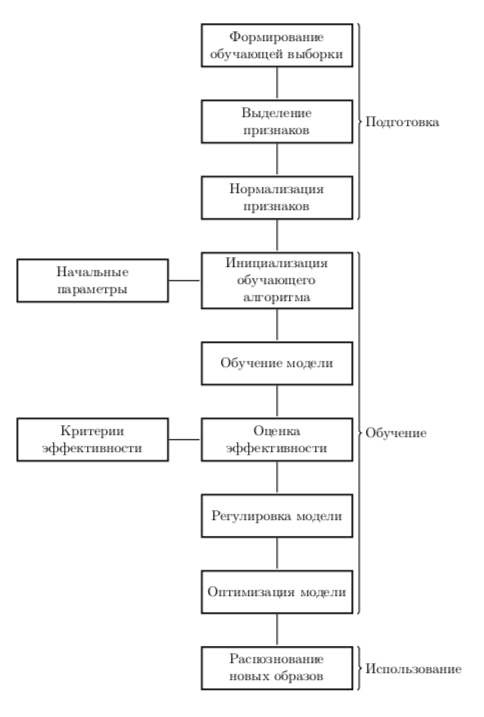
\includegraphics[width=1\textwidth]{figures/SVM_flow.png}
    \caption{Алгоритм обучение}
\end{figure}

После обучения классификатора можно переходить к класификации образов, листинг~\ref{lst:development:classification}. Всего в программном средстве различается 16 типов личности определяющих характеристики.

\lstinputlisting[
    style=commonstyle,
    caption=Пример файла конфигурации модуля,
    label=lst:development:classification
]{src/evaluate_single_instance.java}

Для хранения учетных и пользовательских данных используется СУБД MongoDB. Условно все данные можно разделить на образцы изображений, листинг~\ref{lst:development:json:sample} и описание пользовательских данных, листинг~\ref{lst:development:json:user}. Для хранения используется формат JSON что упрощает преобразование информации при общения сервисов между собой и с клиентом. 

\lstinputlisting[
    style=commonstyle,
    caption=Пример JSON-документа описывающего образец текста,
    label=lst:development:json:sample
]{src/sample_item.json}

\lstinputlisting[
    style=commonstyle,
    caption=Пример JSON-документа описывающего пользователя,
    label=lst:development:json:user
]{src/user_item.json}

Общая диаграмма классов представлена на рисунке~\ref{fig:develoipment:class_fdp}.
\begin{figure}[ht]
    \centering
    \label{fig:develoipment:class_fdp}
    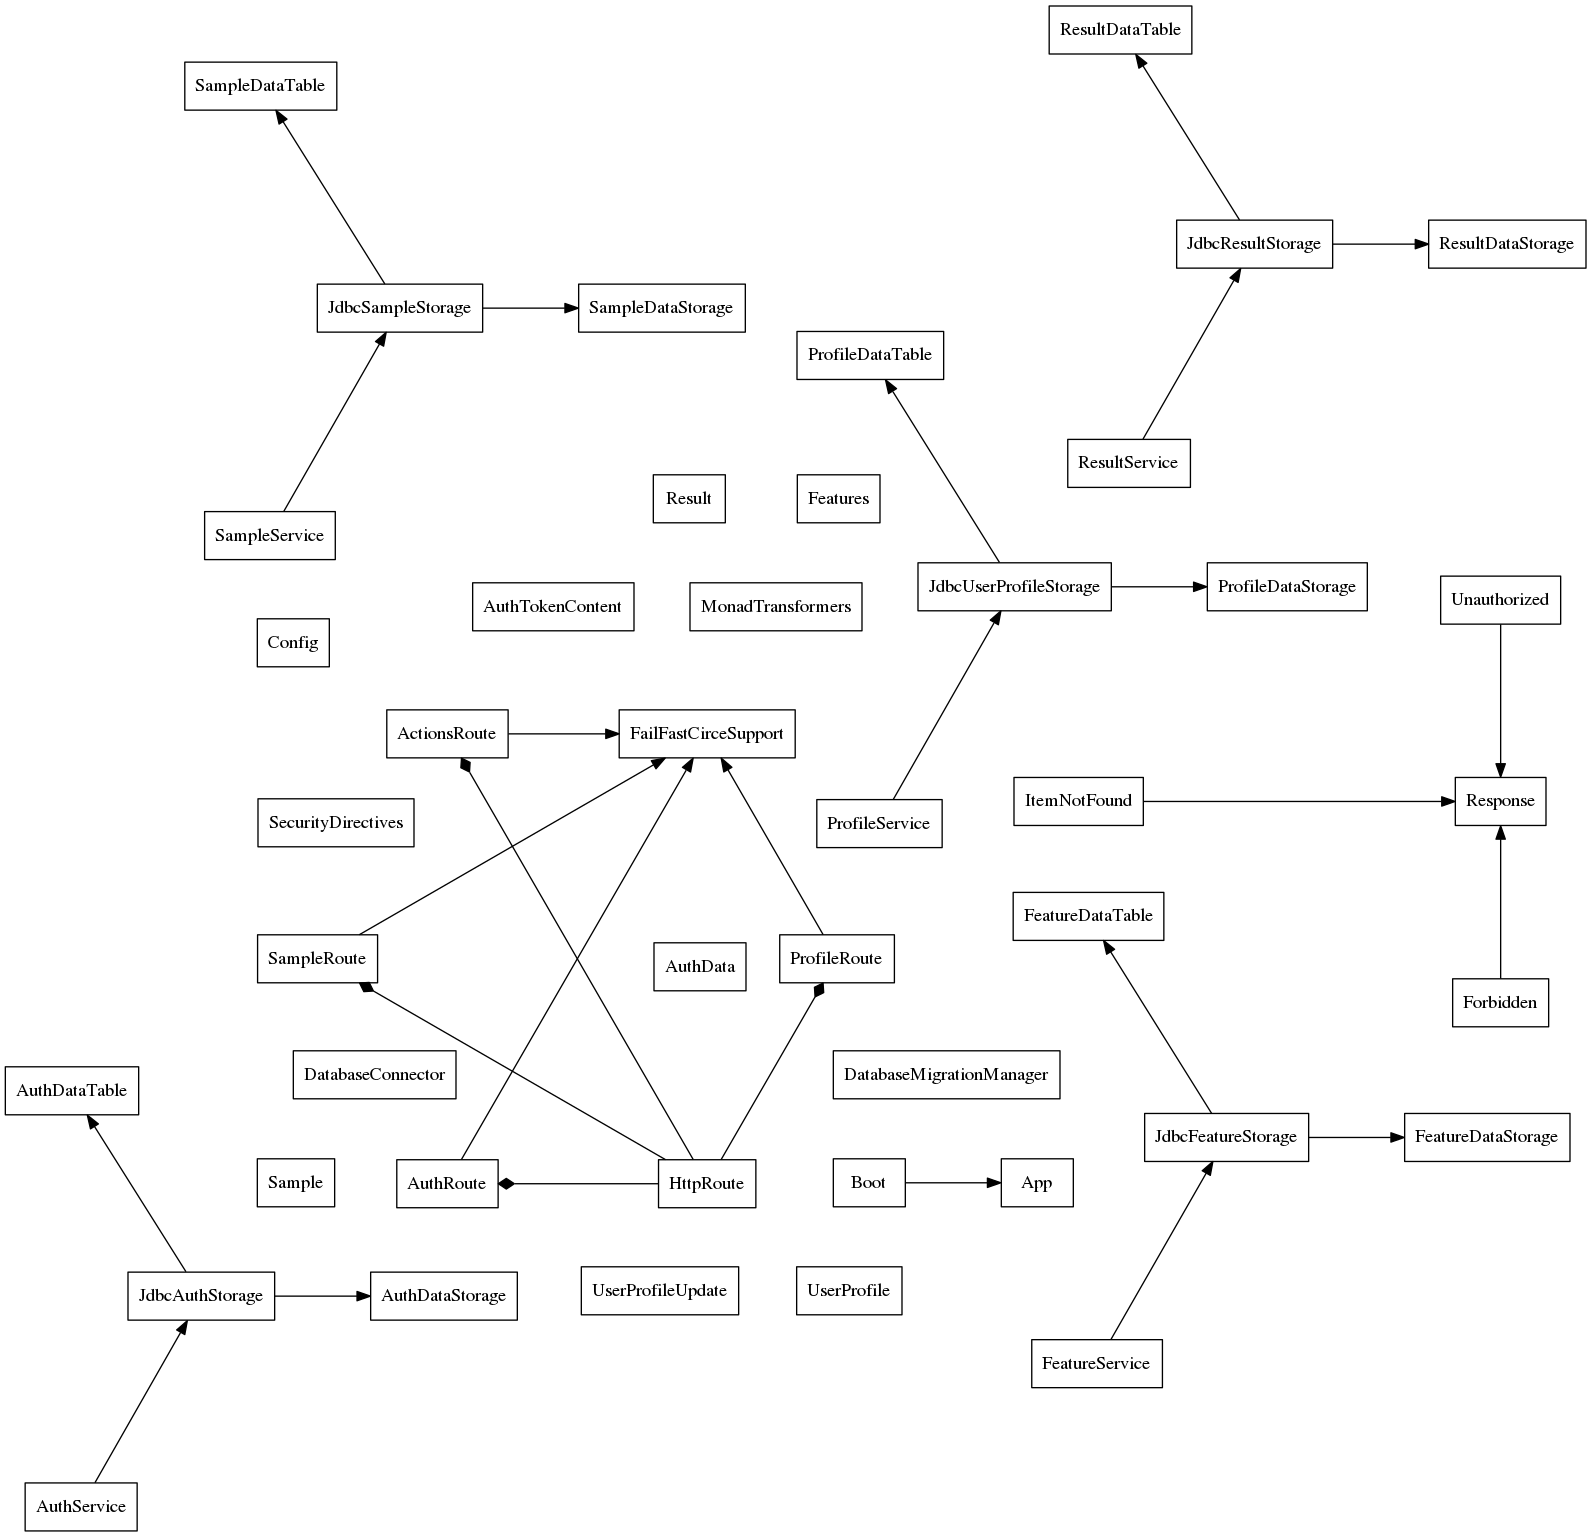
\includegraphics[width=1\textwidth]{figures/classes-fdp.png}
    \caption{Иерархия классов}
\end{figure}